\documentclass[11pt]{article} 
\usepackage[utf8]{inputenc}

%%% PAGE DIMENSIONS
\usepackage{geometry}
\geometry{a4paper}

\usepackage{graphicx} % support the \includegraphics command and options

% \usepackage[parfill]{parskip} % Activate to begin paragraphs with an empty line rather than an indent

%%% PACKAGES
\usepackage{float}
\usepackage{booktabs}
\usepackage{array}
\usepackage{paralist}
\usepackage{verbatim}
\usepackage{subfig} 
\usepackage{fancyhdr}
\usepackage{amsmath}
\usepackage{amssymb}

\pagestyle{fancy} % options: empty , plain , fancy
\renewcommand{\headrulewidth}{0pt} % customise the layout...
\lhead{}\chead{}\rhead{}
\lfoot{}\cfoot{\thepage}\rfoot{}

\usepackage{sectsty}
\allsectionsfont{\sffamily\mdseries\upshape}

\usepackage{listings}
\usepackage{color}

\definecolor{mygreen}{rgb}{0,0.6,0}
\definecolor{mygray}{rgb}{0.5,0.5,0.5}
\definecolor{mymauve}{rgb}{0.58,0,0.82}

\lstset{ 
  backgroundcolor=\color{white},   % choose the background color; you must add \usepackage{color} or \usepackage{xcolor}; should come as last argument
  basicstyle=\footnotesize,        % the size of the fonts that are used for the code
  breakatwhitespace=false,         % sets if automatic breaks should only happen at whitespace
  breaklines=true,                 % sets automatic line breaking
  captionpos=b,                    % sets the caption-position to bottom
  commentstyle=\color{mygreen},    % comment style
  firstnumber=1000,                % start line enumeration with line 1000
  frame=single,	                   % adds a frame around the code
  keepspaces=true,                 % keeps spaces in text, useful for keeping indentation of code (possibly needs columns=flexible)
  keywordstyle=\color{blue},       % keyword style
  language=Python,                 % the language of the code
  numbers=left,                    % where to put the line-numbers; possible values are (none, left, right)
  numbersep=5pt,                   % how far the line-numbers are from the code
  numberstyle=\tiny\color{mygray}, % the style that is used for the line-numbers
  rulecolor=\color{black},         % if not set, the frame-color may be changed on line-breaks within not-black text (e.g. comments (green here))
  showspaces=false,                % show spaces everywhere adding particular underscores; it overrides 'showstringspaces'
  showstringspaces=false,          % underline spaces within strings only
  showtabs=true,                   % show tabs within strings adding particular underscores
  stepnumber=1,                    % the step between two line-numbers. If it's 1, each line will be numbered
  stringstyle=\color{mymauve},     % string literal style
  tabsize=2,	                   % sets default tabsize to 2 spaces
  title=\lstname                   % show the filename of files included with \lstinputlisting; also try caption instead of title
}


\title{Práctica 6: Support Vector Machines}
\author{Ana Martín Sánchez, Nicolás Pastore Burgos}
\date{21/09/2021} 

\begin{document}
\maketitle

\section{Solución propuesta}

\subsection{Resultados obtenidos}

 \begin{figure}[h!]
    \begin{center}
    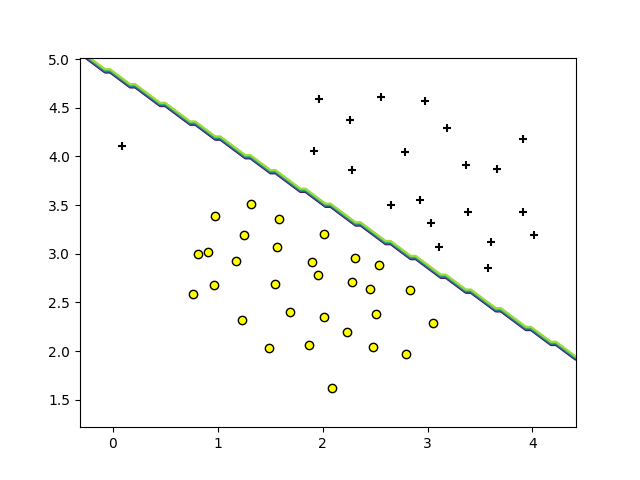
\includegraphics[width=0.45\textwidth]{Figura1.png}
    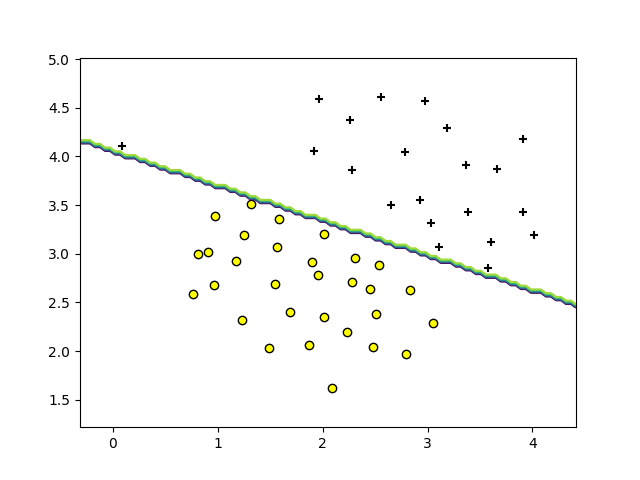
\includegraphics[width=0.45\textwidth]{Figura2.png}
    \end{center}
 \end{figure}

 \begin{figure}[h!]
    \begin{center}
    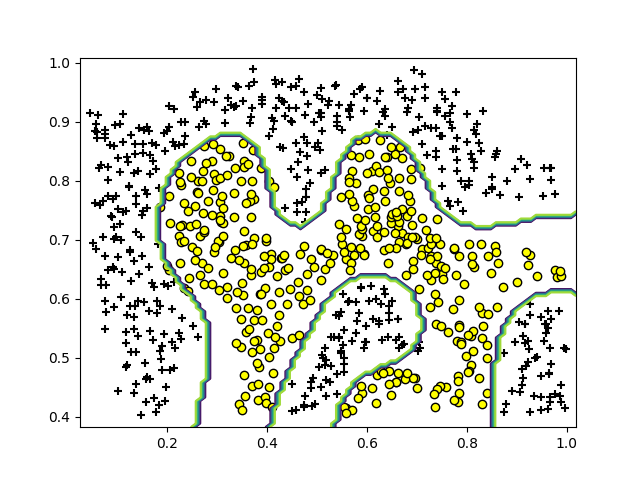
\includegraphics[width=0.45\textwidth]{Figura3.png}
    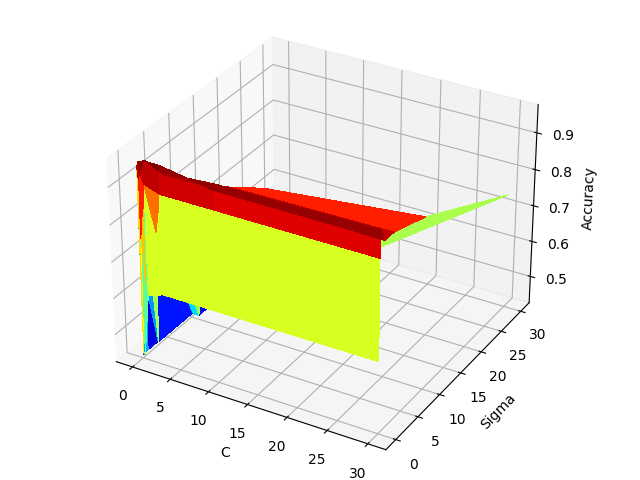
\includegraphics[width=0.45\textwidth]{Figura4.png}
    \end{center}
 \end{figure}

 \begin{figure}[h!]
    \begin{center}
    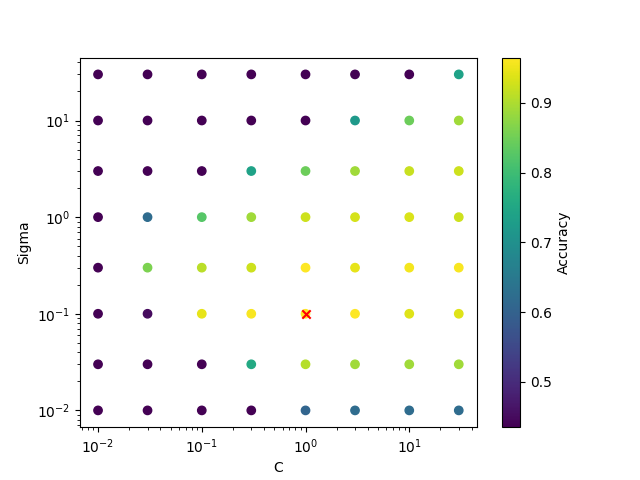
\includegraphics[width=0.45\textwidth]{Figura5.png}
    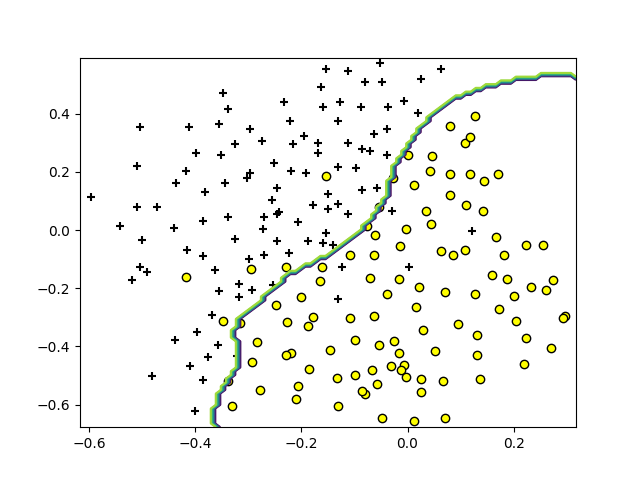
\includegraphics[width=0.45\textwidth]{Figura6.png}
    \end{center}
 \end{figure}

 \begin{figure}[h!]
    \begin{center}
    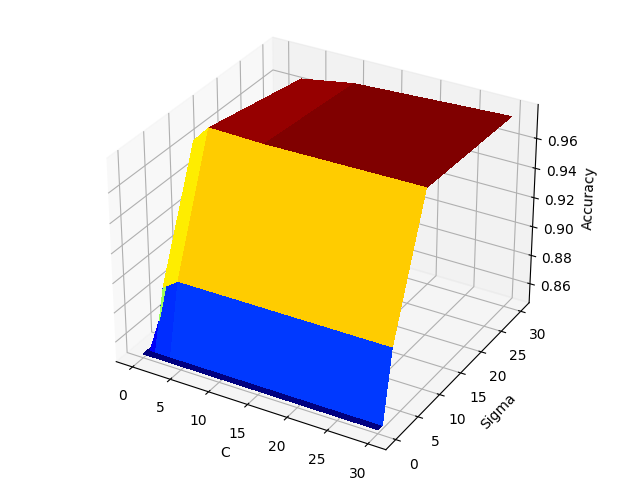
\includegraphics[width=0.45\textwidth]{Figura7.png}
    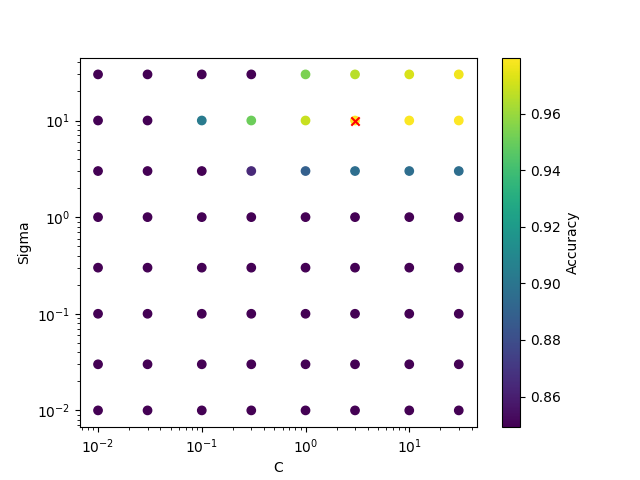
\includegraphics[width=0.45\textwidth]{Figura8.png}
    \end{center}
 \end{figure}



\newpage
\subsection{Implementación}

\lstinputlisting[language=Python]{main.py}


\end{document}
